\draftspread{%
  \begin{paperwidefigure}
% Submission typography; original vector and all geometry retained separately.
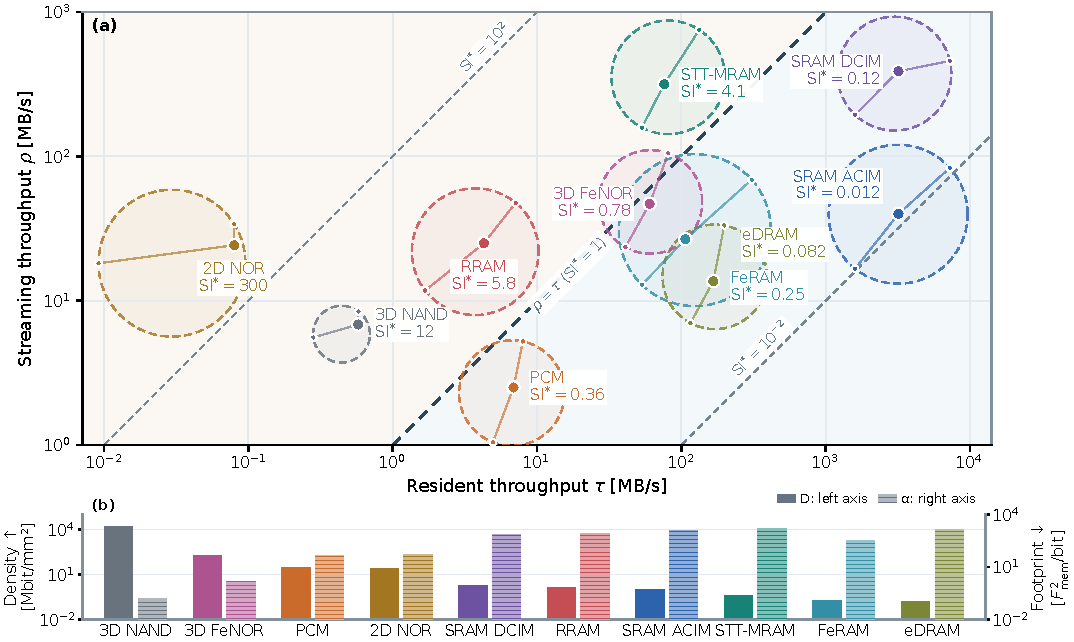
\includegraphics[width=\textwidth]{figures/hardware_capacities_paper.pdf}
\caption{Streaming capacity $\rho$ and resident-update capacity $\tau$ for ten native reference configurations; $1\ \mathrm{MB/s}=10^6\ \Byte/\mathrm{s}$. Large points are typical scenarios; small points preserve the original paired alternatives. Circles summarize only those finite scenarios, and $\RI^*=1$ is a capacity-ratio reference, not a universal workload boundary. Native sizes and resources differ.}
\label{fig:hardware-capacities}
\end{paperwidefigure}

  \par\medskip
  % Selected from Task II(b) 04_crosscheck/data/results.json; no O-projection values are implied.
\begin{paperwidetable}
\caption{Streaming intensities of representative inference matrix stages}
\label{tab:workload-intensity}
\footnotesize\setlength{\tabcolsep}{1.6pt}\renewcommand{\arraystretch}{1.25}
\begin{tabularx}{\textwidth}{@{}p{0.20\textwidth}*{12}{>{\centering\arraybackslash}X}@{}}
\toprule
& \multicolumn{6}{c}{\textbf{Weight projections}} & \multicolumn{6}{c}{\textbf{Attention}} \\
\cmidrule(lr){2-7}\cmidrule(l){8-13}
& \multicolumn{3}{c}{QKV ($U$)} & \multicolumn{3}{c}{FFN/MoE ($U$)} & \multicolumn{3}{c}{Prefill ($L$)} & \multicolumn{3}{c}{Decode ($L$)} \\
\cmidrule(lr){2-4}\cmidrule(lr){5-7}\cmidrule(lr){8-10}\cmidrule(l){11-13}
Model & $1\Kilo$ & $128\Kilo$ & $1\mathrm{M}$ & $16$ & $1\Kilo$ & $16\Kilo$ & $1\Kilo$ & $8\Kilo$ & $64\Kilo$ & $1\Kilo$ & $8\Kilo$ & $64\Kilo$ \\
\midrule
Qwen3.5-2B & 0.200 & 25.6 & 204.8 & 0.00347 & 0.222 & 3.6 & 6.0 & 34.0 & 258.0 & 10.0 & 66.0 & 514.0 \\
Ministral 3 8B & 0.167 & 21.3 & 170.7 & 0.00167 & 0.107 & 1.7 & 10.0 & 66.0 & 514.0 & 18.0 & 130.0 & 1026.0 \\
Qwen3.6-35B-A3B & 0.111 & 14.2 & 113.8 & 0.0130 & 0.833 & 13.3 & 12.0 & 68.0 & 516.0 & 20.0 & 132.0 & 1028.0 \\
Hy3 (295B) & 0.100 & 12.8 & 102.4 & 0.00477 & 0.306 & 4.9 & 20.0 & 132.0 & 1028.0 & 36.0 & 260.0 & 2052.0 \\
Ling-1T (1000B) & 0.100 & 12.8 & 102.4 & 0.00326 & 0.208 & 3.3 & 20.0 & 132.0 & 1028.0 & 36.0 & 260.0 & 2052.0 \\
MiMo-V2.5-Pro (1020B) & 0.0377 & 4.8 & 38.6 & 0.00347 & 0.222 & 3.6 & 35.2 & 214.4 & 1648.0 & 60.8 & 419.2 & 3286.4 \\
\bottomrule\end{tabularx}
\par\smallskip\raggedright
Entries are $\SI$; all roles use one byte/element. QKV includes any gate, excluding O. FFN/MoE counts one dense FFN or one routed expert. Prefill builds KV from empty; decode appends one token to a visible length $L$. $1\Kilo=1024$, $1\mathrm{M}=1024^2$. Ling-1T at $64\Kilo$ uses the fixed extension.
\end{paperwidetable}

}
\section{Hardware and Workload Characterization}
\label{sec:characterization}
\subsection{Memory-Based Reference Configurations}
\outline{Introduce the ten native analog/digital reference configurations in Fig.~\ref{fig:hardware-capacities}, grounded in device and macro sources~\cite{SACIM-03,SDCIM-01,NOR-01,NAND-05,RRAM-01,MRAM-06,PCM-01,FERAM-01,GC-04,FENOR-02} and shared peripheral assumptions~\cite{CMOS-02,CMOS-03,CMOS-07}. Explain the three paired engineering scenarios and complete service accounting, retaining native matrix dimensions, resources, and update organizations. Read absolute capacity and capacity ratio separately; these are literature-grounded estimates rather than equal-area chip comparisons.}
\draftreserve{0.35in}{Native configurations and complete service accounting.}
\draftcolumnbreak
\subsection{Inference Matrix Workloads}
\outline{Use the six fixed model configurations~\cite{qwen35,ministral3,qwen36,hy3,ling,mimo} as structural examples for Table~\ref{tab:workload-intensity}, counting common inputs once per matrix stage at one byte per element. Explain QKV intensity $U/N_{\mathrm{proj}}$ and FFN intensity $U(D+F)/(3DF)$ using output width $N_{\mathrm{proj}}$ (including any gate), hidden width $D$, and dense-FFN or single-expert width $F$. For grouped-query attention, use the native head sharing and possibly unequal query/key and value widths: prefill creates each token's KV once, whereas decode appends one token and treats historical KV as resident.}
